\documentclass[11pt]{article}

\usepackage{amsmath}
\usepackage{graphicx}
\usepackage{subcaption}

\newcommand{\numpy}{{\tt numpy}}    % tt font for numpy

\topmargin -.5in
\textheight 9in
\oddsidemargin -.25in
\evensidemargin -.25in
\textwidth 7in

\begin{document}

% ========== Edit your name here
\author{Aobo Yang (ay6gv)}
\title{CS6316: HW3}
\maketitle

\medskip

% ========== Begin answering questions here
\begin{enumerate}

\item
KNN and Model Selection (k)

1.6
\medskip

The best $k$ is $7$ and the corresponding accuracies are shown in the table below. The reason of that some $k$ works better than others is that $k$ decides the model complexity. Smaller $k$ may make the model too complicate and easier to be affected by noises nearby, so it overfits the training set. Larger $k$, on the other hand, may make the model too generic, so it underfits.

\begin{center}
  \begin{tabular}{ |c|c| }
   \hline
   K & Accuracy \\
   3 & 0.6155 \\
   5 & 0.6275 \\
   7 & 0.629 \\
   9 & 0.626 \\
   11 & 0.6285 \\
   13 & 0.6255 \\
   \hline
  \end{tabular}
\end{center}

1.7
\medskip

The bar graph between $k$ and accuracy is shown in \ref{fig:knn_bar}

\begin{figure}[!h]
  \centering
  \begin{subfigure}[b]{0.4\linewidth}
    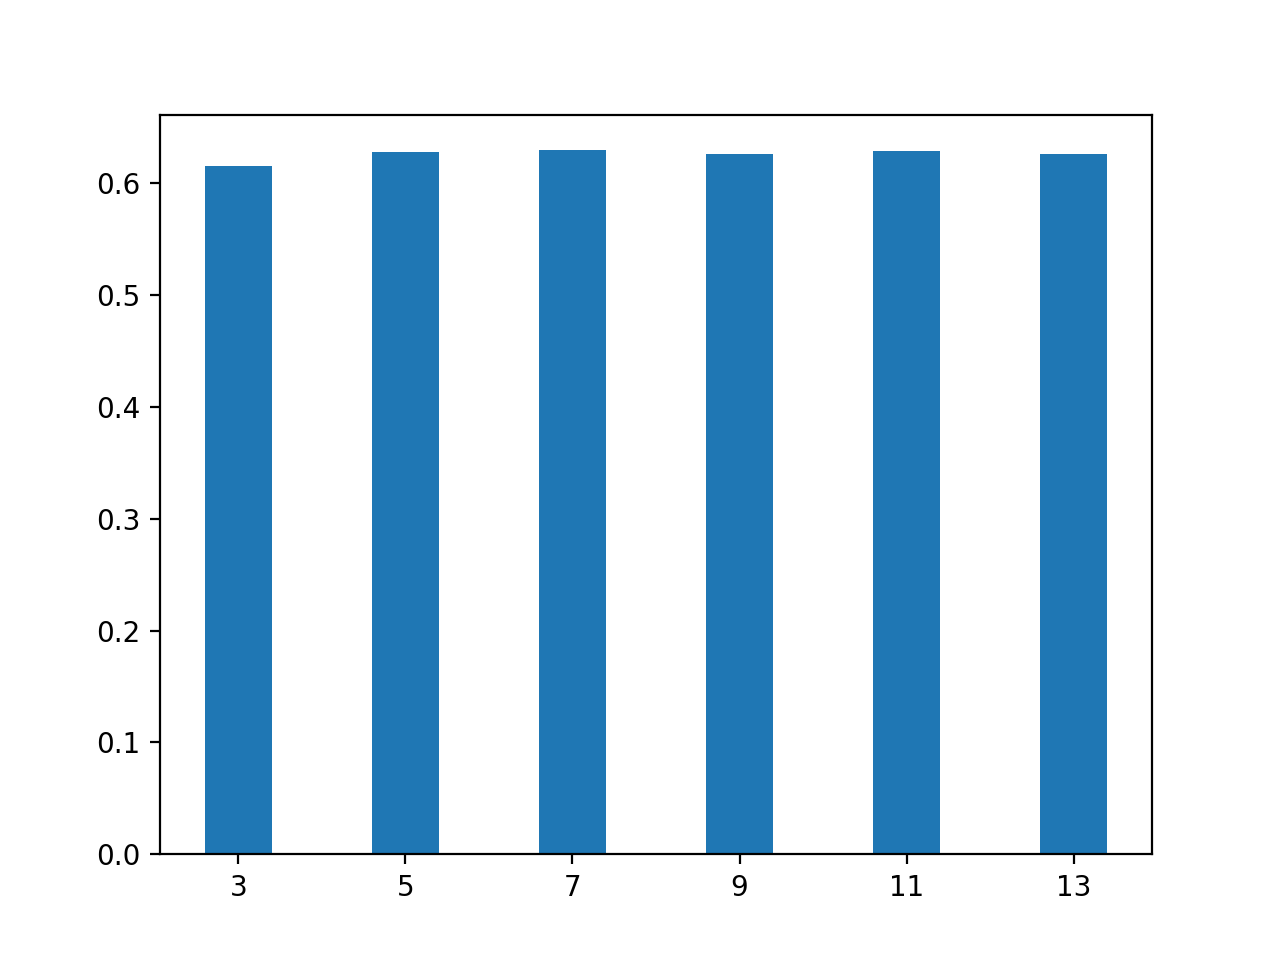
\includegraphics[width=\linewidth]{figures/knn_bar.png}
  \end{subfigure}
  \caption{KNN Bar}
  \label{fig:knn_bar}
\end{figure}


\item
Support Vector Machines

The 3-fold cross-validation accuracies of different hyperparameters are shown in the table below.

\begin{center}
  \begin{tabular}{ |c|c|c|c|c| }
   \hline
    kernel & C & degree & training accuracy & validation accuracy \\
    linear & 1 &  & 0.8522 & 0.8514 \\
    linear & 10 &  & 0.8523 & 0.8516 \\
    linear & 100 &  & 0.8523 & 0.8516 \\
    rbf & 1 &  & 0.8541 & 0.8519 \\
    rbf & 10 &  & 0.8612 & 0.8546 \\
    rbf & 100 &  & 0.8712 & 0.8563 \\
    rbf & 1000 &  & 0.8875 & 0.8495 \\
    poly & 1 & 1 & 0.8504 & 0.8508 \\
    poly & 1 & 3 & 0.8207 & 0.8196 \\
    poly & 1 & 5 & 0.7778 & 0.7775 \\
    poly & 10 & 1 & 0.8521 & 0.8511 \\
    poly & 10 & 3 & 0.8459 & 0.8425 \\
    poly & 10 & 5 & 0.7863 & 0.7849 \\
   \hline
  \end{tabular}
\end{center}

The best performing model is the one with the "rbf" kernel and C value of $100$. It achieves the highest validation accuracy $0.8563$.

\medskip

The data preprocessing contains three steps. First, I use LabelEncoder to map the target labels to $0$ and $1$. Second, I use scikit-learn's StandardScaler to normalize all the continuous attributes by removing the mean and scaling to unit variance. At last, I use scikit-learn's OneHotEncoder to expand all the categorical features except "native-country". I decide to drop the "native-country" because it alone brings in around 40 new one-hot features which dramatically hurts the SVM training speed and I find having it does not contribute much to the prediction.

\item
Sample QA Questions

(a)

False, larger C penalize violations more so there should be less data fall in the smaller margin which means less support vectors. On the contrary, smaller C leads to larger margin so there are more support vectors.

\medskip

(b)

Correct option (1)

\medskip

(c)

(2)  (1)  (3)


% ========== Continue adding items as needed

\end{enumerate}

\end{document}
\grid
\grid
